%% =====================================================================
\section{Experiments}
\label{sec:experiments}

In this section we empirically evaluate the projection-based filter on three standard ANN benchmarks.
Our experiments are designed to answer four questions:
\begin{enumerate}[label=(Q\arabic*),leftmargin=*]
    \item How much distance-computation and wall-clock time does the filter save, and at what cost in construction recall?
    \item How does the filter compare against the obvious alternative of simply reducing the sampling rate of NN-Descent?
    \item Does the empirical behavior of the filter match the $m/d$ break-even condition derived in Section~\ref{sec:breakeven}?
    \item Does the filter compose with RP-tree initialization, and does the construction-recall loss translate into a meaningful search-recall loss on the resulting graph?
\end{enumerate}


\subsection{Setup}
\label{sec:setup}

\paragraph{Datasets.}
We use three standard benchmarks spanning two dimensionality regimes:
\textbf{GIST~1M} ($n=10^6$, $d=960$) and \textbf{GIST~100K} ($n=10^5$, $d=960$), the high-dimensional image descriptor datasets from the ANN-Benchmarks suite, and
\textbf{SIFT~1M} ($n=10^6$, $d=128$), the standard low-dimensional visual-feature benchmark.
GIST serves as the primary testbed because its dimensionality is in the regime where filtering is expected to help; SIFT serves as a stress-test at the other end of the spectrum.

\subsection{Construction Recall vs.\ Search Recall}
\label{sec:construction_recall}

In graph-based ANN, it is important to distinguish between \emph{construction recall} and \emph{search recall}, as they measure fundamentally different quantities.

\textbf{Construction recall} measures the fraction of true $k$-nearest neighbors that appear in each node's neighbor list in the constructed graph:
\begin{equation}
    \text{Recall}_{\text{constr}} = \frac{1}{n} \sum_{i=1}^{n} \frac{|N_G(i) \cap N^*(i)|}{k}
    \label{eq:construction_recall}
\end{equation}
where $N_G(i)$ is the set of $k$ neighbors of point $i$ in the constructed graph and $N^*(i)$ is the set of its true $k$-nearest neighbors computed via brute force.
This metric directly evaluates the quality of the graph construction algorithm---a construction recall of 0.6 means that, on average, 60\% of each node's true nearest neighbors are present in its neighbor list.

\textbf{Search recall}, by contrast, measures the fraction of true $k$-nearest neighbors returned by a search algorithm (such as greedy beam search) that operates on the constructed graph at query time:
\begin{equation}
    \text{Recall}_{\text{search}} = \frac{1}{|\mathcal{Q}|} \sum_{q \in \mathcal{Q}} \frac{|S(q) \cap N^*(q)|}{k}
    \label{eq:search_recall}
\end{equation}
where $\mathcal{Q}$ is the set of queries, $S(q)$ is the set of $k$ results returned by the search algorithm for query $q$, and $N^*(q)$ is the set of true $k$-nearest neighbors of $q$ in the dataset.

A graph with moderate construction recall (e.g., 0.60) can still achieve high search recall (e.g., 0.90+) because the search algorithm explores beyond immediate neighbors through multi-hop greedy traversal, effectively compensating for missing edges in the local neighborhood.
In this work, we primarily report construction recall, as it directly reflects the quality of the graph produced by NN-Descent and is the metric most affected by our filtering approach.

\paragraph{Baseline and filter configuration.}
The baseline is our single-threaded C++ implementation of NN-Descent with \emph{new/old} partitioning, reverse-neighbor expansion, and sampling rate $\rho = 0.5$, running until the relative update fraction falls below $\delta = 10^{-3}$.
Unless stated otherwise we set $k = 10$, max candidates per point $mc = 40$, and for the projection filter $m = 32$ projections.
We sweep the confidence level $p_\tau \in \{0.80, 0.85, 0.90, 0.95, 0.99\}$.
Ground-truth neighbors for recall computation are obtained by brute force on GPU via FAISS.

\paragraph{Metrics.}
(i) The construction recall as defined in Equation~\eqref{eq:construction_recall}, (ii) total number of exact distance computations during the iteration phase, (iii) wall-clock construction time including preprocessing, and (iv) filter rate $f$ (fraction of candidate pairs skipped by the filter).
All timings are wall-clock on a single core; dist.\ comps.\ and recall are deterministic given a fixed seed.
For the GIST~100K and SIFT~1M tables we report the mean over four consecutive runs (discarding a first warmup run) to dampen timing noise; for GIST~1M we report a single run, as the per-run cost is large.

\paragraph{Hardware.}
All experiments are run on a single workstation with an Intel Xeon-class CPU and 64~GB of RAM.
The code is compiled with \texttt{g++ -O3 -march=native} and runs single-threaded throughout; no SIMD-specific tuning is applied to the filter beyond what the compiler auto-vectorizes.

\subsection{Filter Sweep: Time, Recall, and Savings}
\label{sec:main_results}

Figure~\ref{fig:time_vs_recall} summarises the core trade-off on SIFT~1M and GIST~1M with random initialization.
Panel~(a) plots wall-clock construction time against final construction recall as $p_\tau$ is swept from $0.99$ down to $0.60$; each star marks the corresponding no-filter baseline.
Panel~(b) reports the percentage of wall-clock time saved relative to that baseline at every swept $p_\tau$.

\begin{figure*}[t]
    \centering
    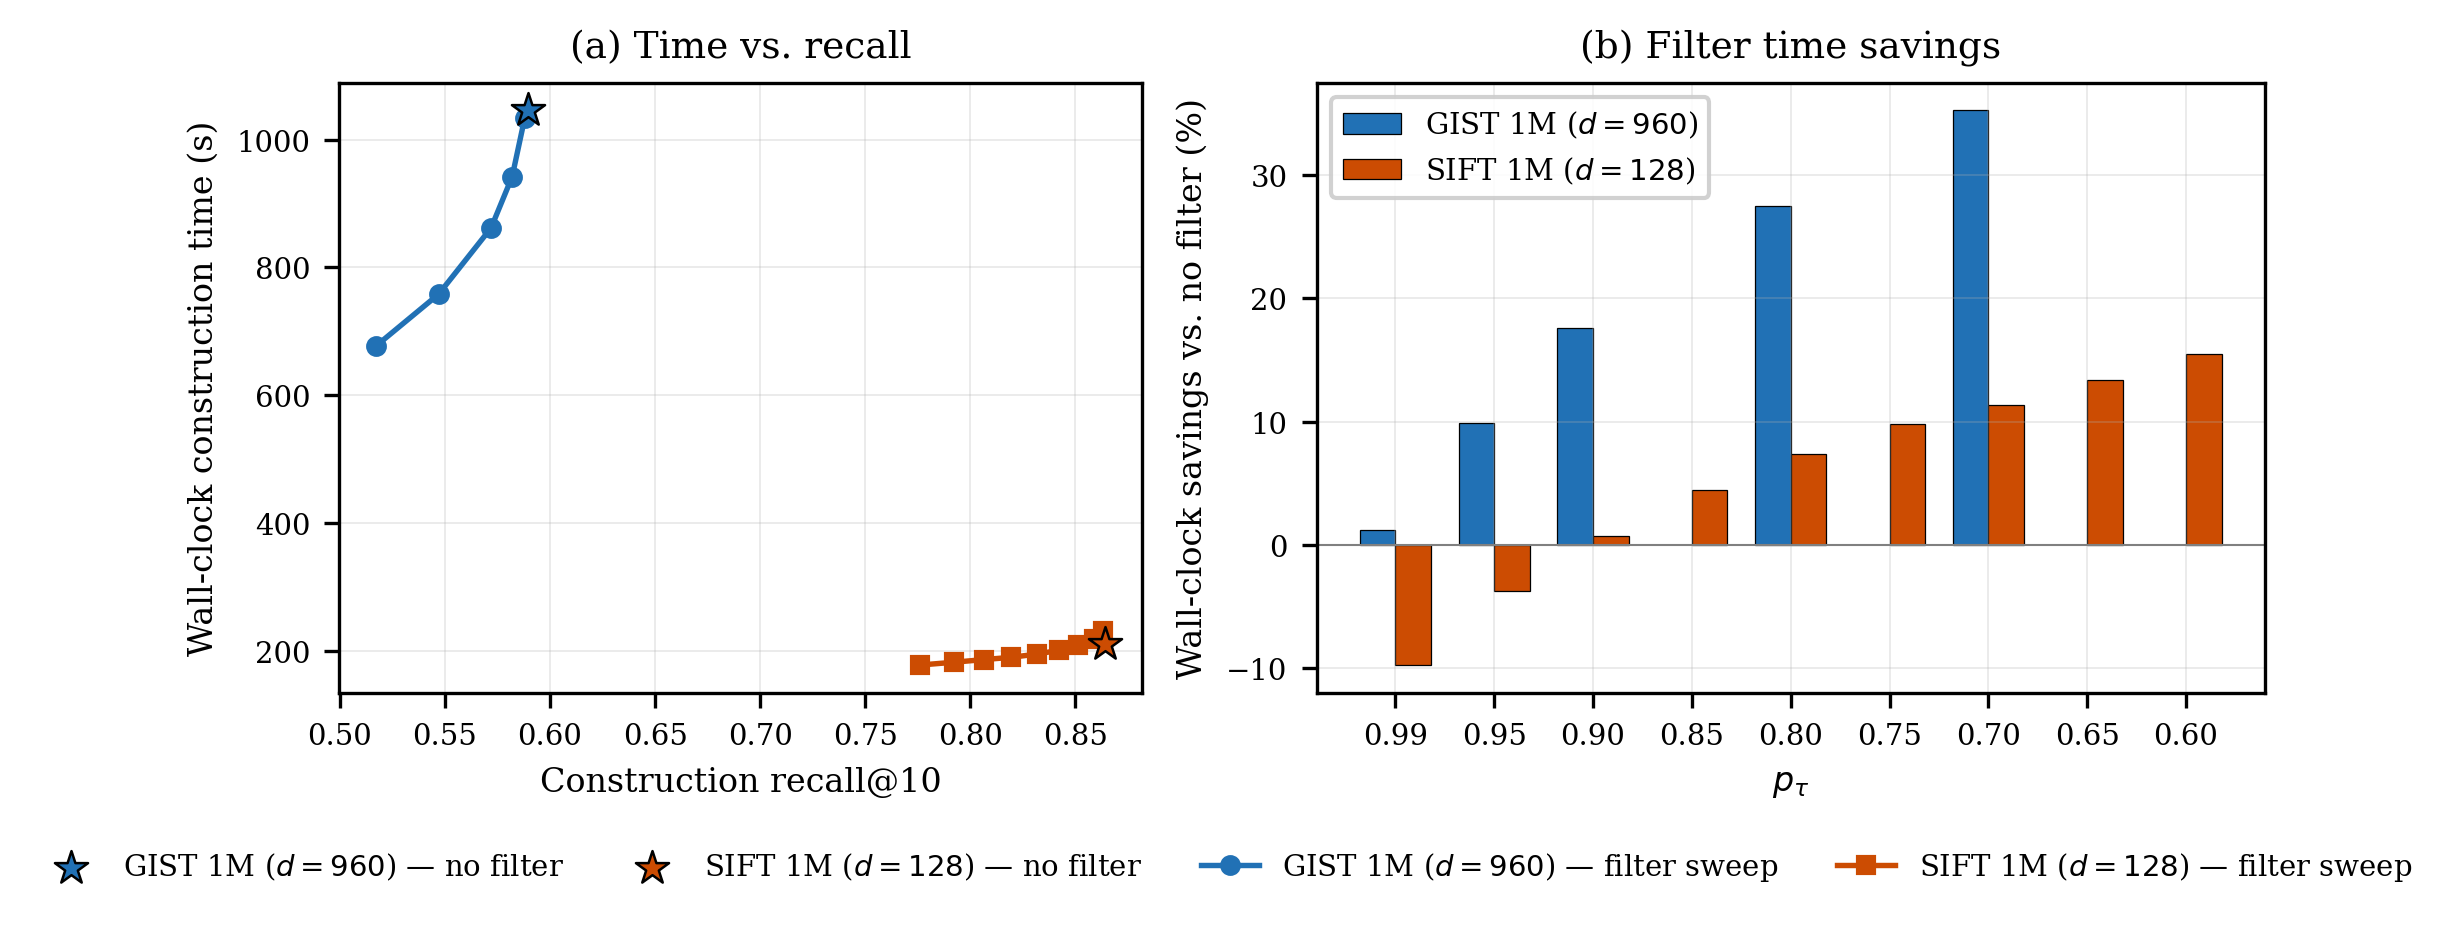
\includegraphics[width=\linewidth]{../report_plots/fig1_time_vs_recall.png}
    \caption{SIFT~1M and GIST~1M with random init.
    (a)~Wall-clock construction time vs.\ construction recall@10 as $p_\tau$ is swept; stars are the no-filter baselines.
    (b)~Wall-clock savings (\%) relative to the no-filter baseline, grouped by $p_\tau$.}
    \label{fig:time_vs_recall}
\end{figure*}

Two trends are immediate.
On GIST~1M the time-vs-recall curve bends sharply toward the lower-left as $p_\tau$ is relaxed: recall drifts down smoothly while wall-clock time falls by tens of percent, so the curve lies well below the no-filter star for every filtered configuration.
On SIFT~1M the corresponding curve is almost horizontal---the filter trades construction recall for essentially no wall-clock gain.
Panel~(b) makes this quantitative: GIST savings grow monotonically with filter aggressiveness, from roughly zero at $p_\tau{=}0.99$ to tens of percent at the most aggressive settings, whereas SIFT savings stay within a few percent of zero (and are occasionally slightly \emph{negative} at conservative $p_\tau$, where the filter does real work but skips too few pairs to pay back its own overhead).
Both behaviours are consistent with the $m/d$ break-even of Section~\ref{sec:breakeven}: for $m{=}32$, GIST ($d{=}960$) sits far on the profitable side of the threshold, while SIFT ($d{=}128$) straddles it.

A second useful observation from panel~(a) is the \emph{shape} of the recall loss.
At the conservative end of the sweep the filter costs very little recall (the curve stays near the no-filter star), and relaxing $p_\tau$ produces gradual, predictable recall drift rather than a cliff.
This gives a clean operating knob: a practitioner can pick the largest $p_\tau$ that produces an acceptable recall loss and claim the corresponding wall-clock savings.

\subsection{Filter vs.\ Sampling Reduction}
\label{sec:filter_vs_mc}

The simplest way to cut distance computations in NN-Descent is to shrink the per-node candidate pool via the $mc$ parameter (maximum candidates per neighbor); a reasonable worry is therefore that our filter is merely re-introducing this knob in disguise.
Figure~\ref{fig:filter_vs_mc} tests this directly on GIST~1M, with random init.
The red curve is the filter sweep ($mc{=}40$, varying $p_\tau$) and the blue curve is the sampling sweep (no filter, varying $mc$).

\begin{figure}[t]
    \centering
    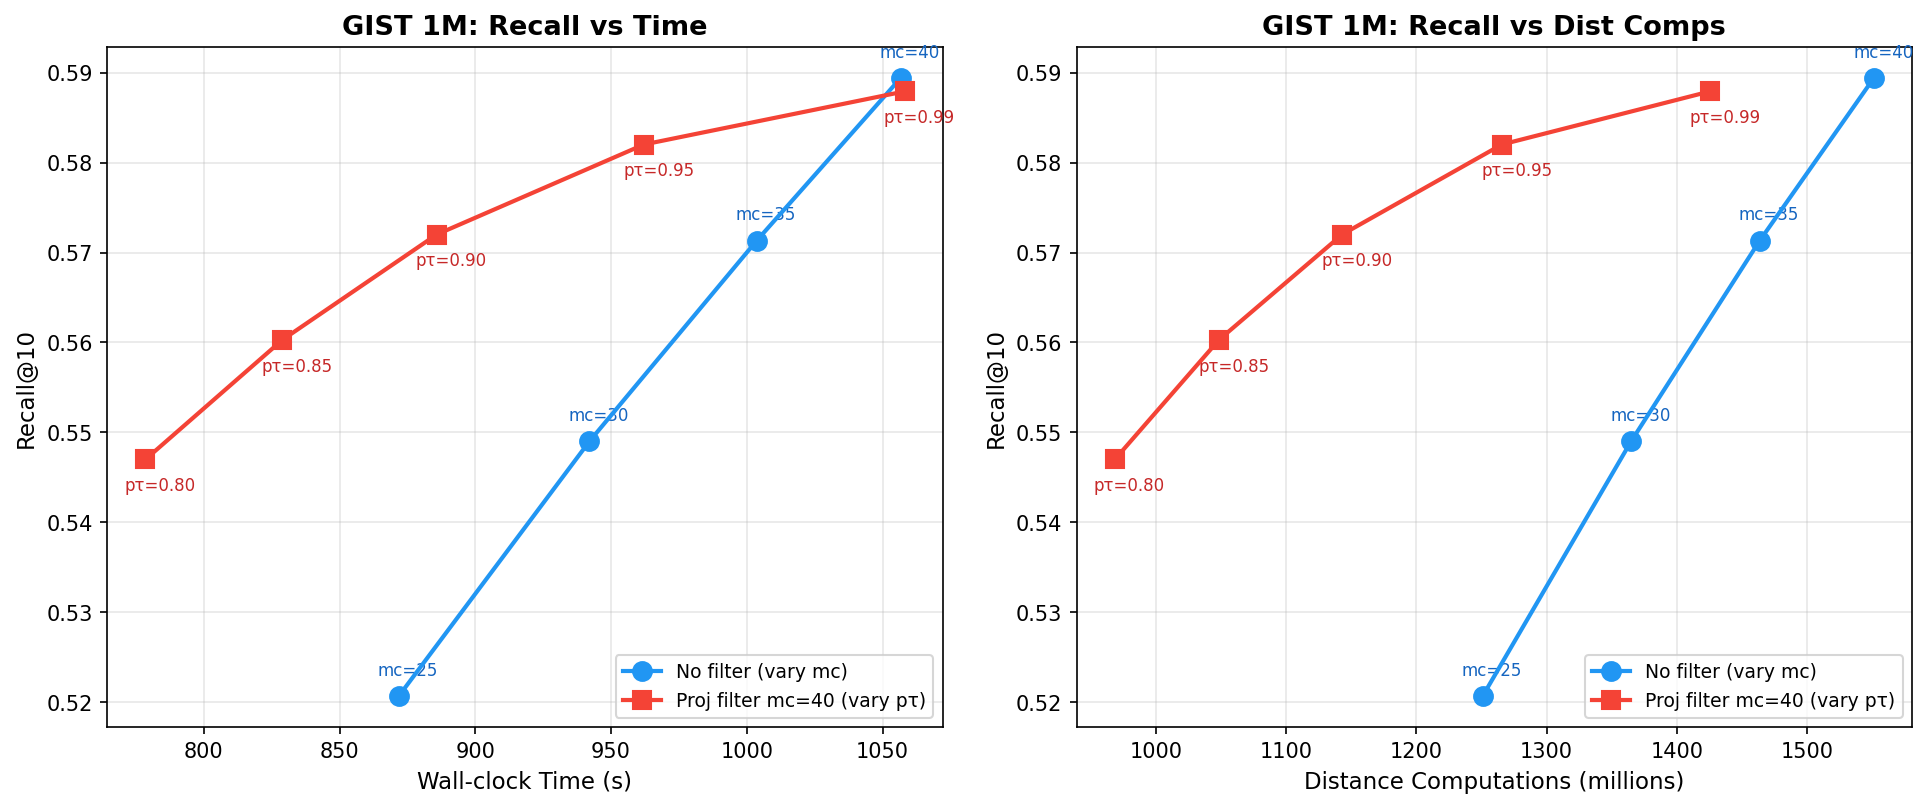
\includegraphics[width=\linewidth]{../report_plots/fig2_filtering_vs_sampling.png}
    \caption{GIST~1M, random init: filter sweep versus sampling ($mc$) reduction.
    (Left) Recall vs.\ wall-clock time.
    (Right) Recall vs.\ distance computations.
    Across both axes the filter curve lies strictly above the sampling curve at every matched budget---cheaper per recall point in both distance computations and wall-clock time.}
    \label{fig:filter_vs_mc}
\end{figure}

The two curves are decisively separated: at every matched budget---whether counted in distance computations (right panel) or in wall-clock seconds (left panel)---the filter curve sits above the $mc$-reduction curve, i.e.\ it delivers strictly higher construction recall for the same cost.
The qualitative reason is structural.
Shrinking $mc$ discards candidate pairs indiscriminately, losing good and bad pairs alike, whereas the projection filter uses a cheap approximate-distance signal to discard pairs that are unlikely to produce an update.
Because that signal is correlated with the true distance, the filtered-out pairs are disproportionately the ones that would not have changed the graph anyway.
The filter is therefore not a rebranded sampling knob; it exploits structural information that uniform subsampling cannot access.
We will extend this comparison to SIFT~1M once the matching sampling sweep completes; current trends already suggest the gap narrows in low dimension, in line with the break-even argument above.

\subsection{Composing with RP-Tree Initialization}
\label{sec:rptree_init}

All results so far use random initialization.
A practically important question is whether the filter still pays off when combined with a stronger initializer---specifically, the RP-tree initialization used by PyNNDescent, which starts the iterations from a partially-built graph.
Figure~\ref{fig:rptree_time_vs_recall} repeats the layout of Figure~\ref{fig:time_vs_recall} but now includes RP-tree curves (dashed, darker) alongside the random-init curves (solid) for both SIFT~1M and GIST~1M.

\begin{figure*}[t]
    \centering
    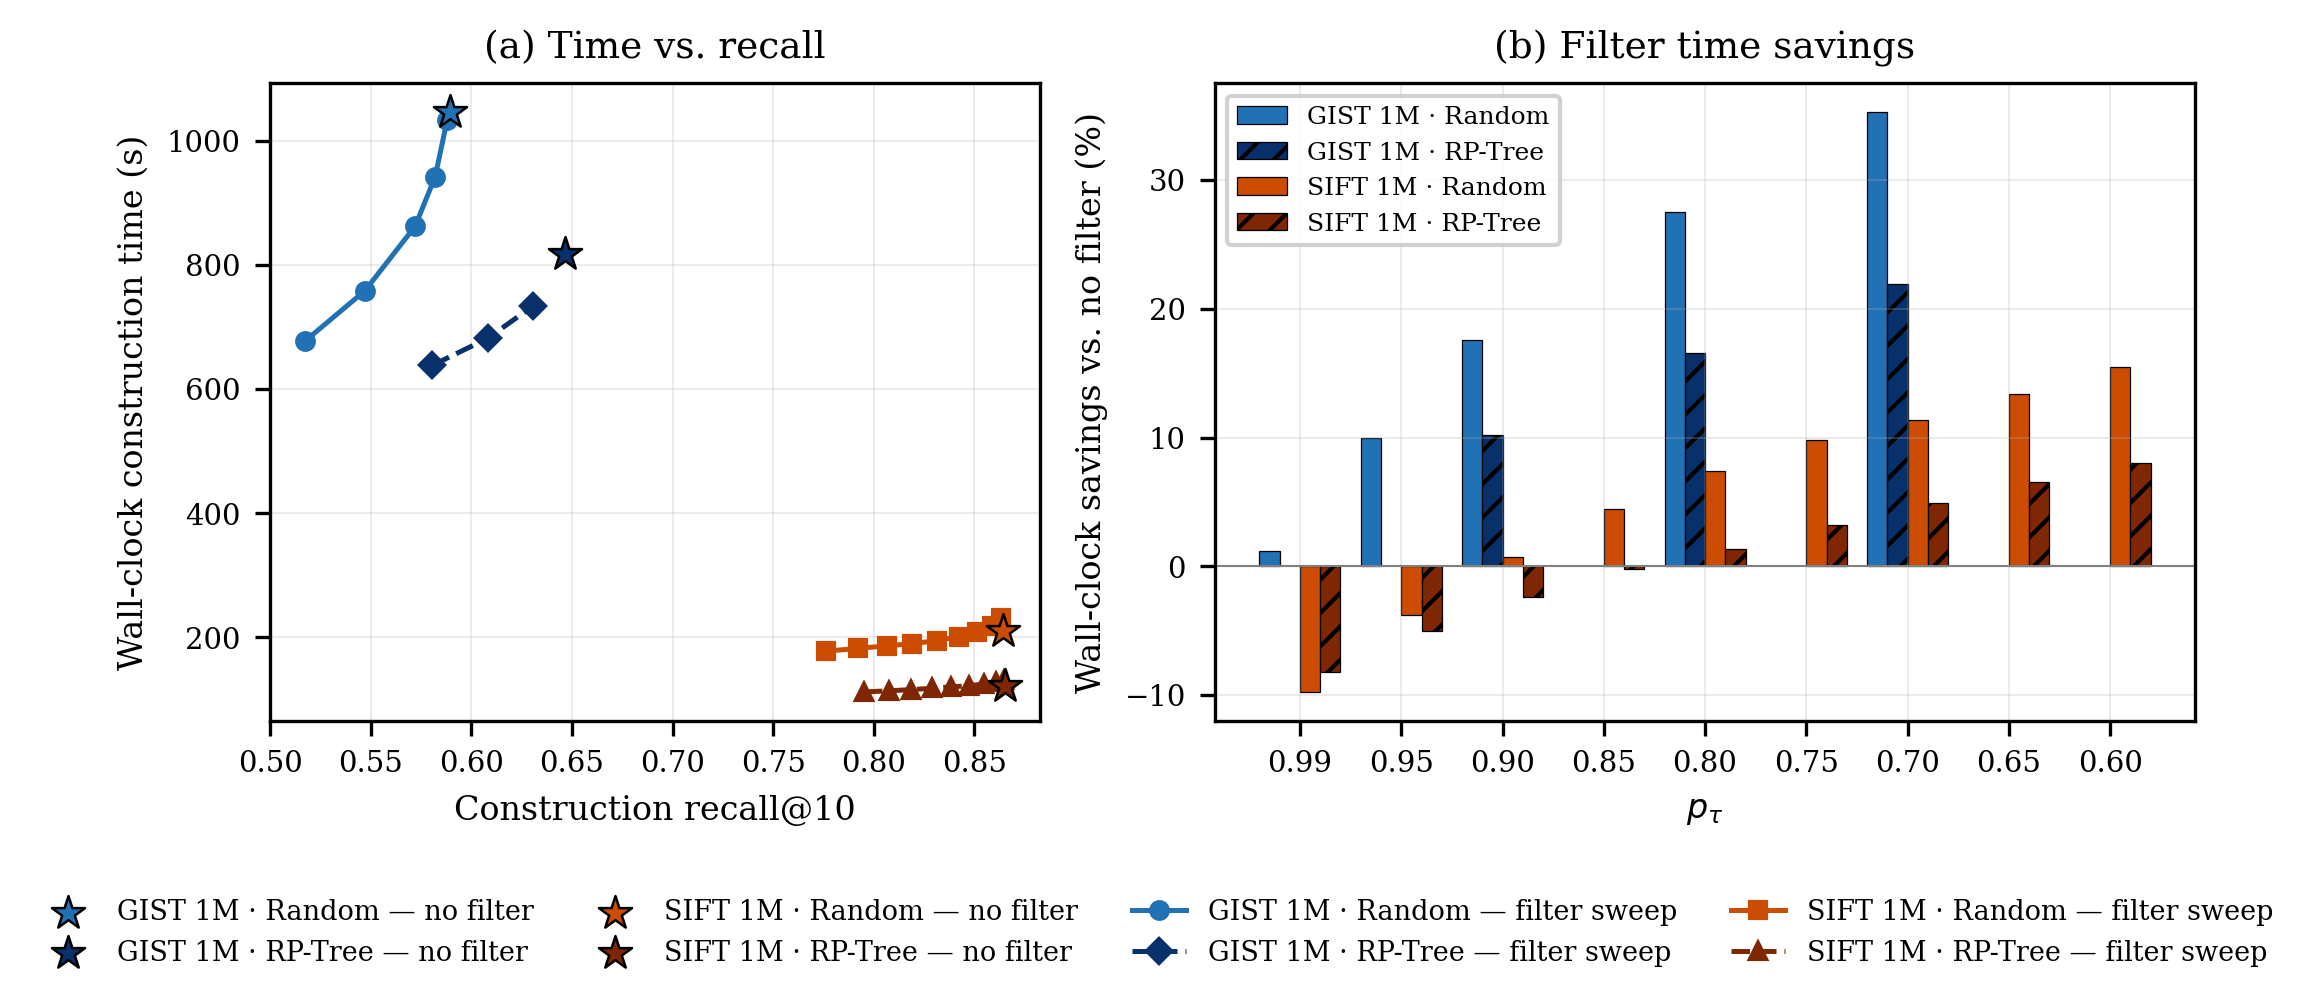
\includegraphics[width=\linewidth]{../report_plots/fig3_rptree_time_vs_recall.png}
    \caption{Same layout as Figure~\ref{fig:time_vs_recall}, adding RP-tree initialization.
    (a)~Wall-clock time vs.\ construction recall for Random (solid) and RP-tree (dashed) init on SIFT~1M and GIST~1M.
    (b)~Wall-clock savings (\%) from the filter, with hatched bars marking RP-tree init.}
    \label{fig:rptree_time_vs_recall}
\end{figure*}

Three trends emerge.
First, RP-tree initialization shifts every no-filter baseline up and to the right in panel~(a): higher final recall at a lower wall-clock time, confirming that a better starting graph shortens the iteration phase.
Second, the filtered RP-tree curve has the same qualitative shape as the random-init curve---relaxing $p_\tau$ smoothly trades construction recall for wall-clock time---so the filter's behavior does not depend on the initializer.
Third, panel~(b) shows that filter savings under RP-tree init are somewhat \emph{smaller} in percentage terms than under random init, especially on GIST.
This is expected and was anticipated in Section~\ref{sec:waste}: RP-tree initialization absorbs the early high-update-rate iterations that offer the most obvious waste for the filter to skip, so the remaining workload is inherently harder to compress further.
Even so, the filter remains clearly profitable on GIST~1M under RP-tree, delivering double-digit percentage savings at moderate $p_\tau$ while preserving the recall advantage that RP-tree brings in the first place.
On SIFT~1M the RP-tree and random-init bars track each other closely and both remain small, again consistent with the $m/d$ break-even.

\subsection{Downstream Search Quality}
\label{sec:search_recall}

Filter savings that come at the cost of user-visible search quality would be a false economy.
To check this, Figure~\ref{fig:search} builds GIST~1M graphs at a representative set of $p_\tau$ values under both initializers and runs a standard greedy beam search with beam width $ef \in \{10, 20, 50, 100, 200\}$.
Each curve is a search-recall vs.\ QPS Pareto front for one built graph.

\begin{figure}[t]
    \centering
    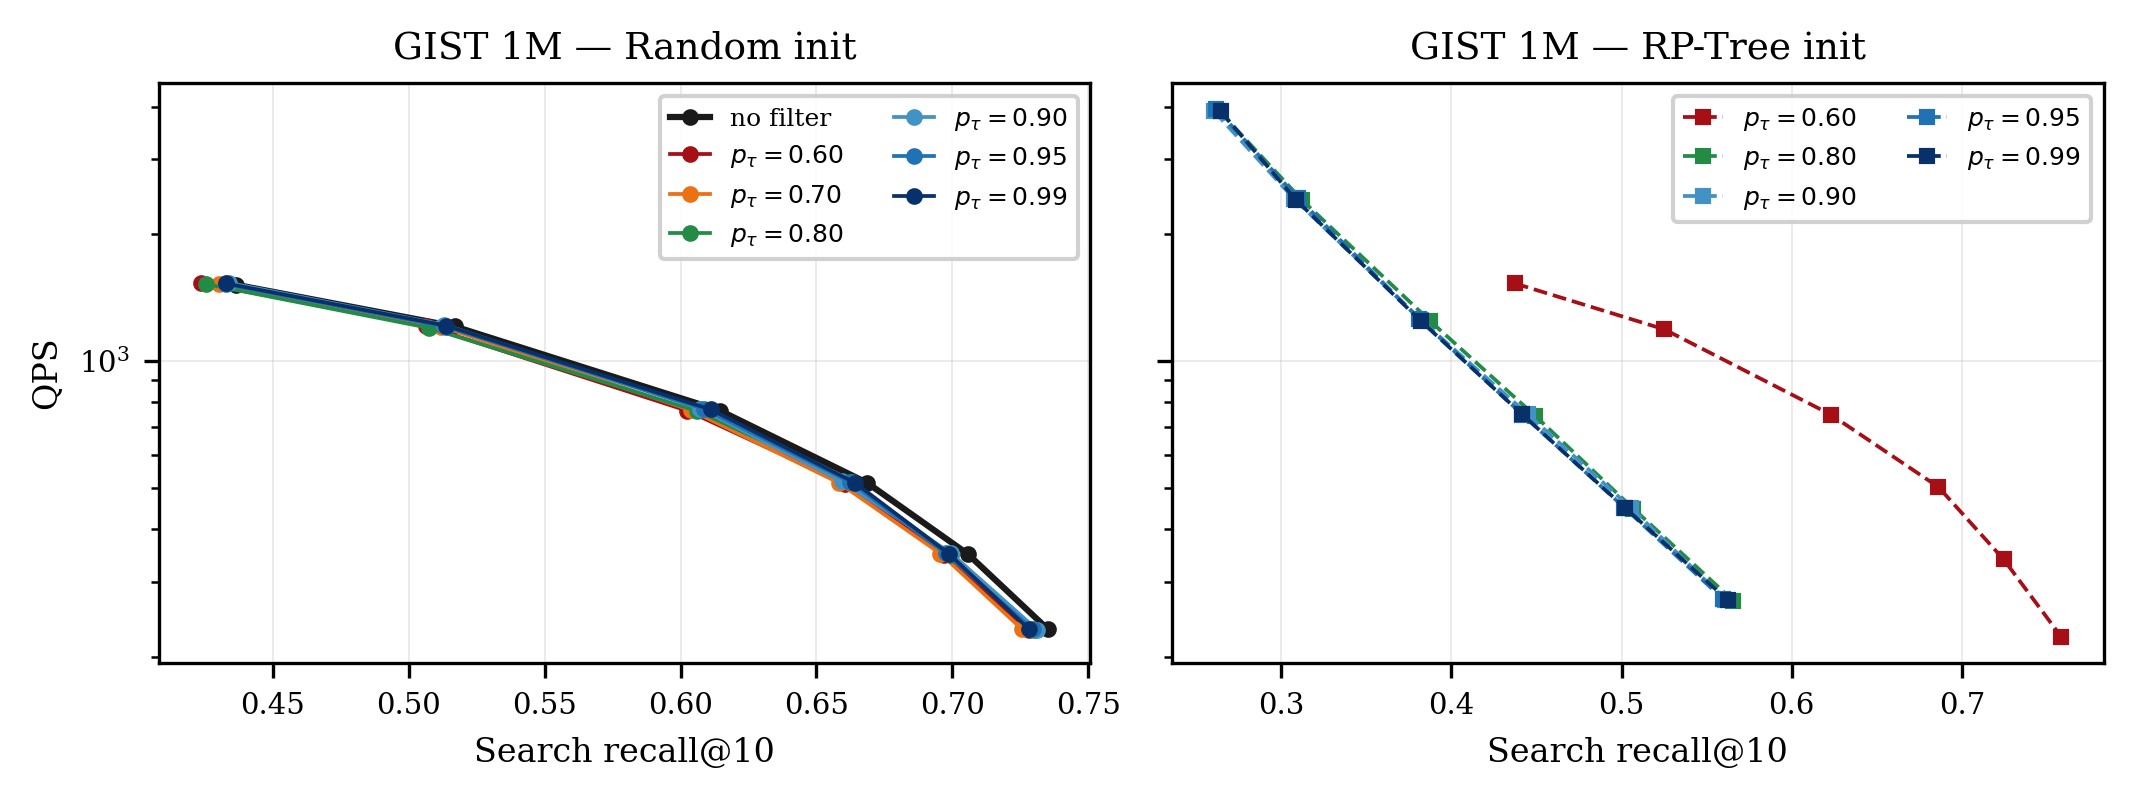
\includegraphics[width=\linewidth]{../report_plots/fig5_search.png}
    \caption{Search recall@10 vs.\ QPS on GIST~1M for graphs built under varying $p_\tau$ (left: random init; right: RP-tree init). Curves for every $p_\tau$ value essentially superimpose on the no-filter curve, showing that the filter's construction-recall cost does not propagate to search quality.}
    \label{fig:search}
\end{figure}

The striking trend is a \emph{collapse}: across the entire $p_\tau$ sweep, and under both initializers, the search-recall/QPS Pareto curves are essentially indistinguishable.
The construction-recall loss we pay in Figures~\ref{fig:time_vs_recall} and~\ref{fig:rptree_time_vs_recall} does not propagate to a downstream search-recall loss of any practical size.
This is consistent with the mechanism reported for other approximate constructions: the edges the filter removes are not random outliers but near-misses that greedy beam search routes around via multi-hop traversal.
The practical implication is the central message of this paper: the construction-time savings demonstrated above are \emph{free} at query time.

\subsection{Summary of Findings}
\label{sec:summary}

We close this section by returning to the four questions of Section~\ref{sec:experiments}.

\paragraph{(Q1) Distance and wall-clock savings vs.\ recall.}
Figure~\ref{fig:time_vs_recall} shows that on GIST~1M the filter trades construction recall for wall-clock time along a smooth, well-behaved curve: relaxing $p_\tau$ produces meaningful double-digit wall-clock savings for a gradual, sub-linear drop in recall, with the no-filter baseline clearly dominated in the $p_\tau{\leq}0.90$ regime.

\paragraph{(Q2) Filter vs.\ sampling reduction.}
Figure~\ref{fig:filter_vs_mc} shows that the filter strictly Pareto-dominates a matched $mc$-reduction sweep on GIST~1M, both in distance computations and in wall-clock time.
The filter is therefore not redundant with a simpler sampling knob; it exploits structural information that uniform subsampling cannot.

\paragraph{(Q3) Dimensionality break-even.}
The SIFT~1M versus GIST~1M contrast in Figures~\ref{fig:time_vs_recall}(b) and~\ref{fig:rptree_time_vs_recall}(b) matches the $m/d$ break-even predicted in Section~\ref{sec:breakeven}: GIST ($d{=}960$) sits well past the break-even and the filter pays off handsomely; SIFT ($d{=}128$) sits near the break-even and the filter gives at most a few percent of wall-clock savings despite cutting distance computations.
This confirms the dimensionality regime where the technique is worth deploying.

\paragraph{(Q4) RP-tree composition and downstream search.}
Figure~\ref{fig:rptree_time_vs_recall} shows that the filter composes cleanly with RP-tree initialization---the same time-vs-recall shape appears, with smaller but still positive wall-clock savings on GIST~1M.
Figure~\ref{fig:search} then shows that none of the construction-recall loss, under either initializer, translates into a measurable loss in downstream search recall.
Taken together, these two results establish that the filter is a drop-in acceleration for realistic NN-Descent pipelines, and that the construction-side savings come essentially for free at query time.

A subset of the GIST~1M $p_\tau$ configurations still need to be re-run with ground truth enabled so that the missing points in Figures~\ref{fig:time_vs_recall}--\ref{fig:rptree_time_vs_recall} can be filled in; we do not expect the trends above to change, but the final draft will incorporate the complete sweep.
